\documentclass[tikz]{standalone}
\usetikzlibrary{calc}
\begin{document}
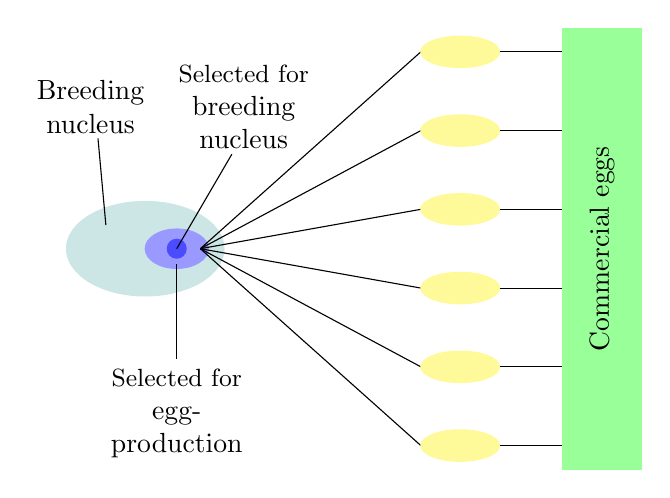
\begin{tikzpicture}
  % Help lines
  %\draw[help lines,step=.2,gray!50] (0,0) grid (8,6);
  %\draw[help lines] (0,0) grid (8,6);
  %\foreach \x in {0, 1, ..., 8} \node[below, gray!50] at (\x,0){\tiny{\x}};
  %\foreach \y in {1, 2, ..., 6} \node[left, gray!50] at (0,\y){\tiny{\y}};
  \draw[fill, teal!20!white] (1.5, 3) ellipse (1 and .6);
  \draw[fill, blue!40!white] (1.9, 3) ellipse (.4 and .25);
  \draw[fill, blue!70!white] (1.9, 3) circle (0.12);
  \node[right, align=center] at (0, 4.8) {Breeding\\nucleus};
  \node[right, align=center] at (1.8, 4.8){\small Selected for\\breeding\\nucleus};
  \node[below, align=center] at (1.9, 1.6){\small Selected for\\egg-\\production};
  \foreach \y in {0.5, 1.5, ..., 5.5}{
    \draw(2.2, 3) -- (5, \y);
    \draw[fill, yellow!40!white] (5.5, \y) ellipse (.5 and .2);
    \draw(6, \y) -- (6.8, \y);
  }
  \draw[fill, green!40!white](6.8, 5.8) rectangle (7.8, 0.2);
  \node[rotate=90] at (7.3, 3){Commercial eggs};
  \draw(1.9,2.8)--(1.9, 1.6);
  \draw(2.6, 4.2)--(1.9, 3);
  \draw(0.9, 4.4)--(1.0, 3.3);
\end{tikzpicture}
\end{document}
